
%%% Local Variables:
%%% mode: latex
%%% TeX-master: t
%%% End:

\documentclass[12pt]{article}

% Housekeeping
\usepackage{amsmath}
\usepackage{amssymb}
\usepackage{gensymb}  % For celsius degree symbol

\usepackage{cite}
\usepackage{algorithmic}

% Theorem config
\usepackage{ntheorem}
\newtheorem{Law}{Law}

\usepackage{array}

\usepackage{xcolor}
\usepackage{listings}
% \lstset{breaklines}	
\lstset{
numbers=left,
numberstyle=\tiny,
%commentstyle=\color{red!50!green!50!blue!50},
% rulesepcolor=\color{red!20!green!20!blue!20},escapeinside=``,
%xleftmargin=2em,
%xrightmargin=2em,
%aboveskip=1em,
backgroundcolor=\color{red!3!green!3!blue!3},
basicstyle=\small\ttfamily,
stringstyle=\color{purple},
keywordstyle=\color{blue!80}\bfseries,
commentstyle=\color{olive}}

\usepackage{graphicx}
\graphicspath{{./}{./Figure/}}
\usepackage{url}

% This should be put last.
\usepackage{hyperref}



\begin{document}
% Life is fucking awesome in the United Arab Emirates!
\title{UCC501 Homework 3 Solutions}
\author{Yanan Xiao
\\\url{http://yxiao.org}}
\maketitle{}
% Fuck that.



\emph{Programming should be fun. So it is with education.}
\section{Why Hydropower Works?}
\label{sec:why-hydropower-works}

\subsection{Return Period}
\label{sec:return-period}

\begin{itemize}
\item Yes.
\item Philosophically we would say that \textbf{nothing is
    impossible}. A more mathematical explanation goes as follows.
\item According to Wikipedia, the return period is defined as such,
\begin{verbatim}
A return period, also known as a recurrence interval (sometimes 
repeat interval) is an estimate of the likelihood of an event, such 
as an earthquake, flood or a river discharge flow to occur. It is a
statistical measurement typically based on historic data denoting the
average recurrence interval over an extended period of time, and is
usually used for risk analysis (e.g. to decide whether a project
should be allowed to go forward in a zone of a certain risk, or to
design structures to withstand an event with a certain return
period). The following analysis assumes that the probability of the
event occurring does not vary over time and is independent of past
events. 
\end{verbatim}
  To simplify our analysis, we follow the assumption that the
  probability of the event occurring does not vary over time and is
  independent of past events.
\item Given that the return period of a flood is 50 years, we have the
  probability of it as such:
  \begin{equation}
    \label{eq:1}
    p=\frac{1}{50}=0.02
  \end{equation}
  Since in a year whether there is a flood or not is \textbf{mutex},
  we have 
  \begin{equation}
    \label{eq:2}
    q = 1-p = 0.98
  \end{equation}
  Following the definition of
  \textbf{Combination\footnote{\url{https://en.wikipedia.org/wiki/Combination}}},
  we calculate the probability of a 50-year flood occurs in two
  consecutive years as follows:
  \begin{equation}
    \label{eq:3}
    P~=~C^{49}_{1}*0.02^{2}*0.98^{48}
  \end{equation}
  where $C^{49}_{1}$ indicates 49 out of 50 slots the two
  \textbf{consecutive} events (in this case, floods)
  reside. Evaluating equation~\eqref{eq:3} we have
  $P=0.0074$. Apparently it's a positive number, so it is possible.
\end{itemize}

\subsection{Within 20 Years}
\label{sec:within-20-years}

\begin{itemize}
\item Intuitively speaking, the answer should be $20\%$. Let's prove
  that. 
\item The definition of recurrence interval is
  \begin{equation}
    \label{eq:4}
    RI~=~\frac{n+1}{m}
  \end{equation}
  where $n$ is number of years on record and $m$ is the number of
  recorded occurrences of the event being considered.
\item Then the probability calculation of this question is equivalent
  to ``How likely for a ball to fall into one of the first 20 boxes,
  given that it is equally likely to fall into any one of 100
  boxes''. Mathematically speaking,
  \begin{equation}
    \label{eq:5}
    P~=~1-(0.01)^{20}
  \end{equation}
  Evaluating equation~\eqref{eq:5} we can get $P=0.18$.
\end{itemize}

\subsection{Does it rain often?}
\label{sec:does-it-rain}

\begin{itemize}
% \item Life is fucking awesome in the United Arab Emirates!
\item We extract the rainfall data manually to one column, then use
  MATLAB to do the remaining data processing (or information
  retrieval, machine learning whatsoever). If the data sheet is too
  big, we will use MATLAB directly to extract information.
\item Following the code implemented in \texttt{rain.m} we can get
  \textbf{Annual Maximum Series} as follows:
\begin{verbatim}
  Columns 1 through 16

  130.6000  101.3000  118.3000  109.0000  110.2000  166.8000
  179.6000  125.8000  195.6000  152.3000  120.1000  147.8000
  141.0000  156.5000  132.6000  153.9000

  Columns 17 through 21

  156.4000  161.9000  158.5000  168.2000  183.7000
\end{verbatim}
  with the plotted figure shown as below,
  \begin{figure}
    \centering
    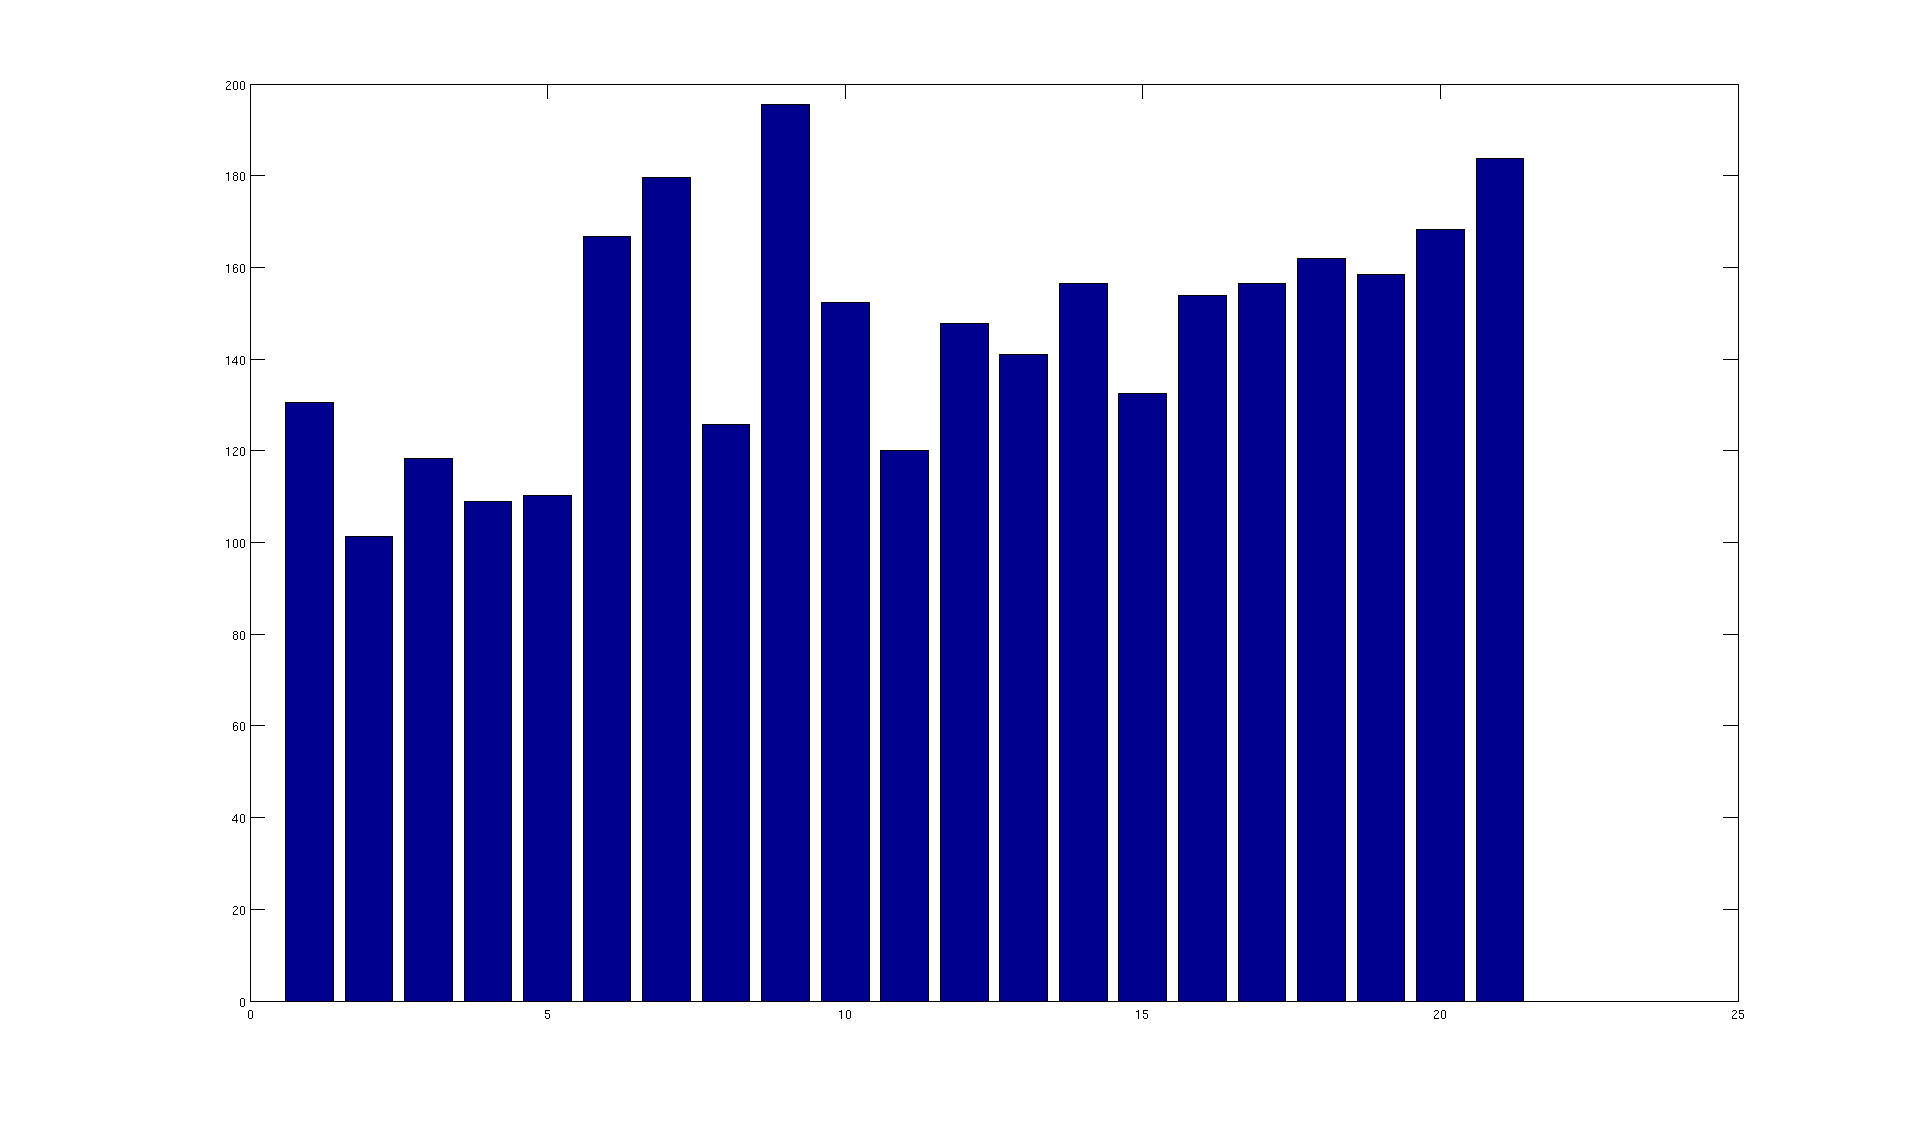
\includegraphics[angle=90,scale=0.4]{annums_bar.png}
    \caption{Annual Maximum Series}
    \label{fig:rain-ams}
  \end{figure}

\item The Gringorten formula is described as such,
  \begin{equation}
    \label{eq:6}
    T=\frac{n+0.12}{i-0.44}
  \end{equation}
  % As we can see from figure~\ref{fig:rain-ams}, $i=9$ when sorted the
  % Annual Maximum Series. Moreover, $n=21$ indicates the years
  % considered. With these values we evaluate equation~\eqref{eq:6}
  % could get $T=2.4673$.
% \item Since $T=2.4673$ we can get probability of occurrence
%   $P=\frac{1}{T}$, thus $P=0.4053$.
% \item The value should be BALABALA, since we require a $50\%$
%   probability of exceedance.
  From $P=\frac{1}{T}$ we get
  \begin{equation}
    \label{eq:13}
    P=\frac{i-0.44}{n+0.12}
  \end{equation}
\item Put all these equations into MATLAB codes, we can get the
  probability of recurrence as follows:
\begin{verbatim}

  Columns 1 through 16

    0.0265    0.0739    0.1212    0.1686    0.2159    0.2633
    0.3106    0.3580    0.4053    0.4527    0.5000    0.5473
    0.5947    0.6420    0.6894    0.7367

  Columns 17 through 21

    0.7841    0.8314    0.8788    0.9261    0.9735

\end{verbatim}
\item The return periods are just the reverse of probability of
  recurrence, as per below.
\begin{verbatim}
Columns 1 through 16

   37.7143   13.5385    8.2500    5.9326    4.6316    3.7986
    3.2195    2.7937    2.4673    2.2092    2.0000    1.8270
    1.6815    1.5575    1.4505    1.3573

  Columns 17 through 21

    1.2754    1.2027    1.1379    1.0798    1.0272
\end{verbatim}
\item 
  \begin{figure}
    \centering
    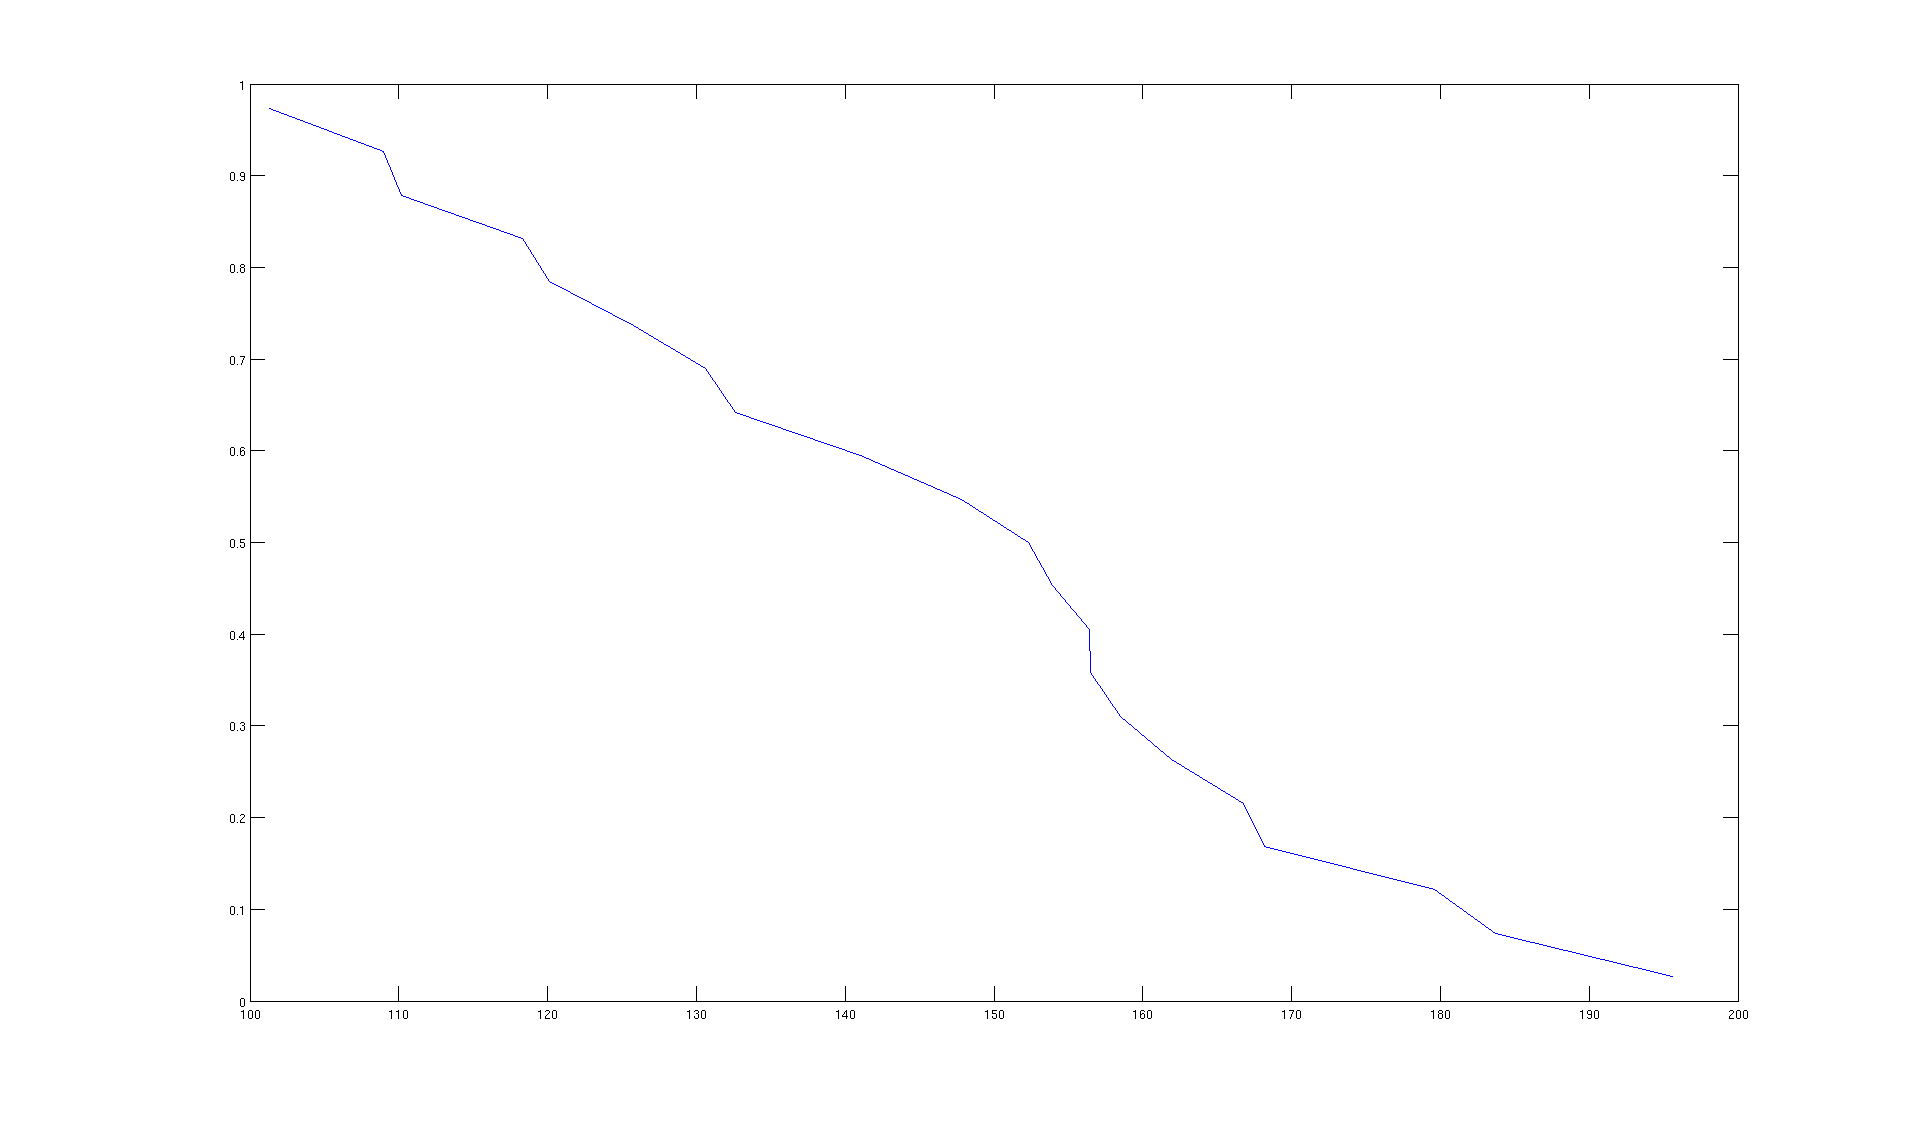
\includegraphics[angle=90,scale=0.4]{rain2}
    \caption{Probability of Recurrence}
    \label{fig:prob-recur}
  \end{figure}
  Therefore from figure~\ref{fig:prob-recur} we can infer $145.7mm$ is
  the rainfall of $50\%$ exceedance.
\end{itemize}

\section{Gone with the Wind}
\label{sec:it-there.-air}

\subsection{The good, The bad}
\label{sec:good-bad}

\begin{itemize}
% \item Life is fucknig awesome in the United Arab Emirates!
\item The pros of utilizing wind energy may be plotted as follows:
  \begin{itemize}
  % \item Life is fucknig awesome in the United Arab Emirates!
  \item Before the death of sun, this type of energy is
    \textbf{renewable}.
  \item In the ``Subsidy Free'' scenario, the levelized cost of wind
    energy is cheap among other renewable energy
    types\footnote{\url{http://www.e3s-center.org/pubs/227/1-13Majumdar.pdf},
      page 16}. 
  \item New types of wind farms like the offshore one levitate the
    issue of high land cost and noise.
  \end{itemize}
\item I would like to list the cons here.
  \begin{itemize}
  \item When built on land, the noise of mainstream wind farm is
    annoying. Therefore, residents could be against the whole building
    plan. 
  \item This type of energy generation is heavily climate, or rather
    geologically dependent. 
  \item The maintenance of wind farms are difficult when compared with
    traditional fossil and hydro power plant.
  \end{itemize}
\item \textbf{I think utilizing wind energy is generally
    viable}.  Though I am a big fan of SciFi and nuclear energy, I
  would say wind energy is viable. As the research and development of
  wind energy goes, there are turbines in use that can make the
  ``most'' of wind, namely the low speed wind. This is important
  because the majority part of the world do not ``enjoy'' high wind
  speed, when the low-speed wind are available to use, due to the
  almost no cost nature of wind, it can generate highly competitive
  electricity, in terms of price.
\end{itemize}

\subsection{How Powerful Could Wind Be?}
\label{sec:how-powerful-could}

\begin{itemize}
\item From the conditions (parameters, configurations, etc) we have,
  we can calculate the \textbf{blade tip speed} using the equation
  below.
  \begin{equation}
    \label{eq:7}
    u~=~\frac{v_{rotation}*\pi*D}{60}
  \end{equation}
  where $D$ is the diameter of the turbine. We have $L=60m$ for blade
  length. Under the assumption that $D=2*L$ we can evaluate
  equation~\eqref{eq:7}, getting $u=24\pi ms^{-1}$.
\item After the first step, we have $u=24\pi$ and $v=15$, we can
  evaluate equation~\eqref{eq:8} to get tip speed ratio.
  \begin{equation}
    \label{eq:8}
    \lambda=\frac{u}{v}
  \end{equation}
  $\lambda=5.0265$, where $v$ stands for wind speed.
\item From the figure given in this question we can infer (well,
  roughly since the exact function of that curve is not
  presented. Somehow if we do want we can do \textbf{curve fitting})
  $C_{p}=0.275$.
\item From the general (namely, \textbf{ideal}) wind power calculation
  formula~\eqref{eq:9} we know how to calculate the power of a wind
  turbine.
  \begin{equation}
    \label{eq:9}
    P~=~\frac{1}{2}\rho Av^{3}C_{p}
  \end{equation}
  Therefore we pre-calculate $A$ as $A=\pi L^{2}$. Evaluating the
  whole formula we can get (as can be verified from MATLAB codes)
  $P=6.2136MW$. Given air pressure and air temperature we use the
  $\rho$ value from corresponding wiki
  page\footnote{\url{https://en.wikipedia.org/wiki/Density_of_air}}. 
\item For power density we only need to reform equation~\eqref{eq:9}
  as follows.
  \begin{equation}
    \label{eq:10}
    PD=P/A~=~\frac{1}{2}\rho v^{3}
  \end{equation}
  Put what we have into this function (in some manner, this equation
  can be regarded as a function. In this case, it's regarding $A$, the
  area a turbine blade swept.) $PD=2.0*10^{-3}MW\cdot m^{-2}$.
\item For this question we just evaluate our MATLAB codes. Total power
  should be $9.7976*10^{8}MJ$.
\end{itemize}

\section{How Did the Red Sun Arise?}
\label{sec:how-did-red}

\subsection{All Solar Leads to Energy}
\label{sec:all-solar-leads}

\begin{itemize}
\item The major difference lies in the way to capture the solar power
  and transform it into electricity---which is at least one of the
  building blocks of modern industry.
\item Solar Photovoltaic does the transformation directly by way of
  semiconductors. The key part is that when temperature rises, the
  electron jumps out of its default orbit therefore forms the current.
\item Concentrating Solar Power (CSP) does the transformation to
  electricity in a passive way. The intermediate part is mechanical,
  like turbines or other engines. 
\end{itemize}

\subsection{Is Solar Energy Really the Ultimate Solution?}
\label{sec:solar-energy-really}

\begin{itemize}
\item Let the solar array size be $x$, then following the assumption
  given in this question, we have
  \begin{equation}
    \label{eq:11}
    x*4.5*365*0.7~=~11000*0.6
  \end{equation}
  Solve this equation we get $x=5.7404$.
\item Since the present technology (as given in question, those solar
  panels in lab are \textbf{way too} expensive) requires us to put 5
  solar panels to generate $1kW$ power, we need $5*x$ solar
  panels. Evaluating the function we get $28.7019$, in practice it
  should be $29$ or $30$ solar panels to meet the need.
\end{itemize}


\section{Chernobyl}
\label{sec:chernobyl}

\subsection{Smaller than Smaller}
\label{sec:smaller-than-smaller}

\begin{itemize}
\item To be short and in Dr. Youssef's rhetoric, fussion is ``marriage''
  and fission is ``divorce''.
\item To be specific, Fission is a reaction when the nucleus of an
  atom, having captured a neutron, splits into two or more nuclei, and
  in so doing, releases a significant amount of energy as well as more
  neutrons.  Fusion is a process where nuclei collide and join
  together to form a heavier atom, usually deuterium and tritium. When
  this happens a considerable amount of energy gets released at
  extremely high
  temperatures\footnote{\url{http://www.iea.org/topics/nuclearfissionandfusion/}}. 
\end{itemize}

\subsection{Decay, Mortal and Immortal}
\label{sec:decay-mort-immort}

\begin{itemize}
\item $^{245}_{96}Cm\rightarrow ^{243}_{94}Pu~+~^{4}_{2}He$ The so
  called alpha stuff is just $^{4}_{2}He$.
\item $^{139}_{51}Sb$
\item For this problem let the initial quantity be $N_{0}$ and
  half-life quantity be $N_{\frac{1}{2}}$, half-life of half-life
  quantity be $N_{\frac{1}{4}}$. Therefore we should be able to get
  equations as follows, where $\lambda$ is a constant, $t_{1}$ and
  $t_{2}$ are the corresponding time to decay.
  \begin{equation}
    \label{eq:12}
    \begin{split}
      N_{\frac{1}{2}} & = e^{-\lambda t_{1}}\\[4pt]
      N_{\frac{1}{4}} & = e^{-\lambda t_{2}}
    \end{split}
  \end{equation}
\item According to the question, we normalize the parameters, where
  $N_{\frac{1}{2}}=\frac{1}{2}$ and $N_{\frac{1}{4}}=\frac{1}{4}$ and
  $t_{1}=28.8$, solve equation~\eqref{eq:12} we get $t_{2}=57.6$ years.
\end{itemize}
\end{document}

